\section{Modificacion de la Interfaz de usuario}


\begin{frame}
\frametitle{Carpetas del proyecto}
\begin{columns}
\column{0.75\linewidth}
Carpetas y archivos importantes
\begin{itemize}
\item \textit{Manifest} - Por el momento es de interes
\item \textit{Java} - C\'odigo fuente - Dentro hay un archivo \textit{MainActivity.kt}
\item \textit{Res} - Recursos (im\'agenes) y definici\'on de interfaces. Dentro hay una carpeta llamada \textit{layout}, con un archivo \textit{activity\_main.xml}
\end{itemize}
\column{0.25\linewidth}
\begin{center}
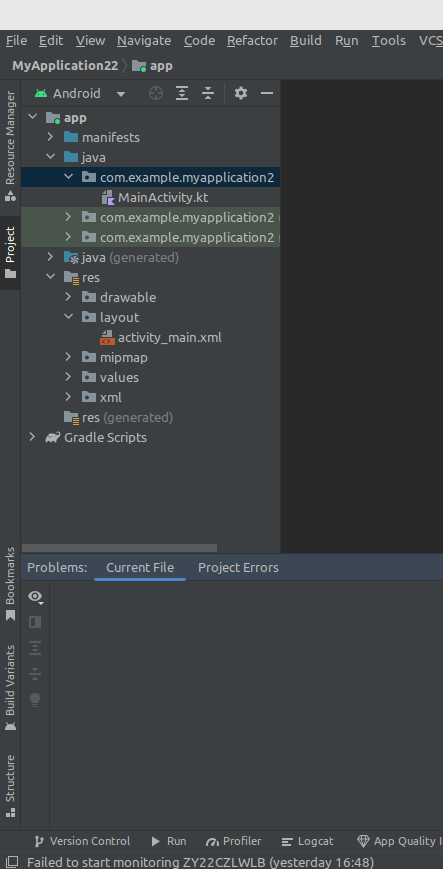
\includegraphics[width=0.95\linewidth]{00_Modificacion/PanelCarpetas.png}    
\end{center}
\end{columns}   
\end{frame}


%\section{Agregar Codigo a la Interfaz}
\begin{frame}[fragile]
\frametitle{Agregar codigo a la interfaz}  


\begin{columns}

\column{0.50\linewidth}
\textit{Apariencia}
\begin{block}{Archivo \textbf{activity\_main.xml}}
\begin{minted}[linenos,fontsize=\tiny]{xml}
<?xml version="1.0" encoding="utf-8"?>
<androidx.constraintlayout.widget.ConstraintLayout 
    xmlns:android="http://schemas.android.com/apk/res/android"
    xmlns:app="http://schemas.android.com/apk/res-auto"
    xmlns:tools="http://schemas.android.com/tools"
    android:layout_width="match_parent"
    android:layout_height="match_parent"
    tools:context=".MainActivity">
    <TextView
        android:layout_width="wrap_content"
        android:layout_height="wrap_content"
        android:text="Hello World!"
        app:layout_constraintBottom_toBottomOf="parent"
        app:layout_constraintEnd_toEndOf="parent"
        app:layout_constraintStart_toStartOf="parent"
        app:layout_constraintTop_toTopOf="parent" />
</androidx.constraintlayout.widget.ConstraintLayout>
\end{minted}

\end{block}

\column{0.48\linewidth}
\textit{Comportamento}
\begin{block}{Archivo \textbf{MainActivity.kt}}
\begin{minted}[linenos,fontsize=\tiny]{kotlin}
package com.example.primeraplicacionandroid
import androidx.appcompat.app.AppCompatActivity
import android.os.Bundle
class MainActivity : AppCompatActivity() {
    override fun onCreate(savedInstanceState: Bundle?) {
        super.onCreate(savedInstanceState)
        setContentView(R.layout.activity_main)
    }
}
\end{minted}
\end{block}
\end{columns}
\end{frame}

\begin{frame}
\frametitle{Interfaz de Usuario}  

\begin{columns}

\column{0.60\linewidth}
\begin{itemize}
\item Define los controles de interfaz que la aplicacion muestra
\item Estos controles pueden estar agrupados en contenedores
\item El archivo \textbf{activity\_main.xml} es la definicion del layout (la organizacion de dichos componentes)
\end{itemize}

\begin{columns}
\column{0.50\linewidth}
\begin{center}
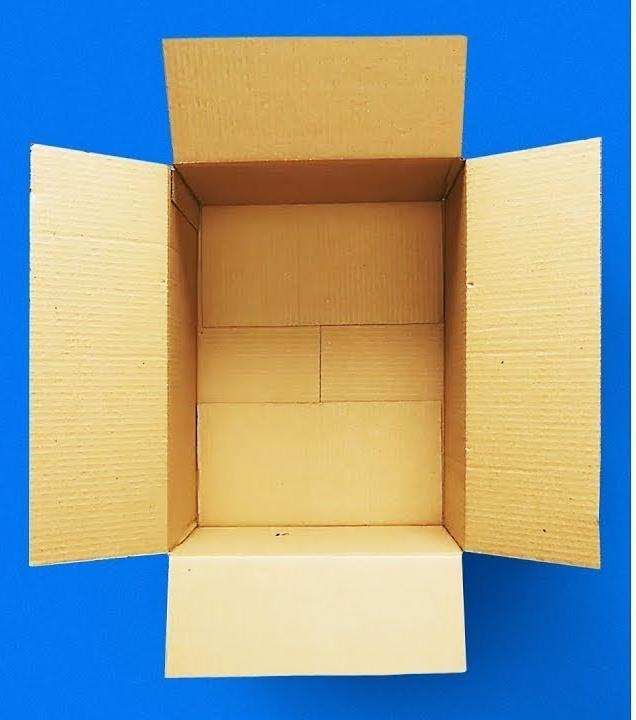
\includegraphics[width=0.75\linewidth]{00_Modificacion/CajaContenedora.png}    
\end{center}
\column{0.50\linewidth}
\begin{center}
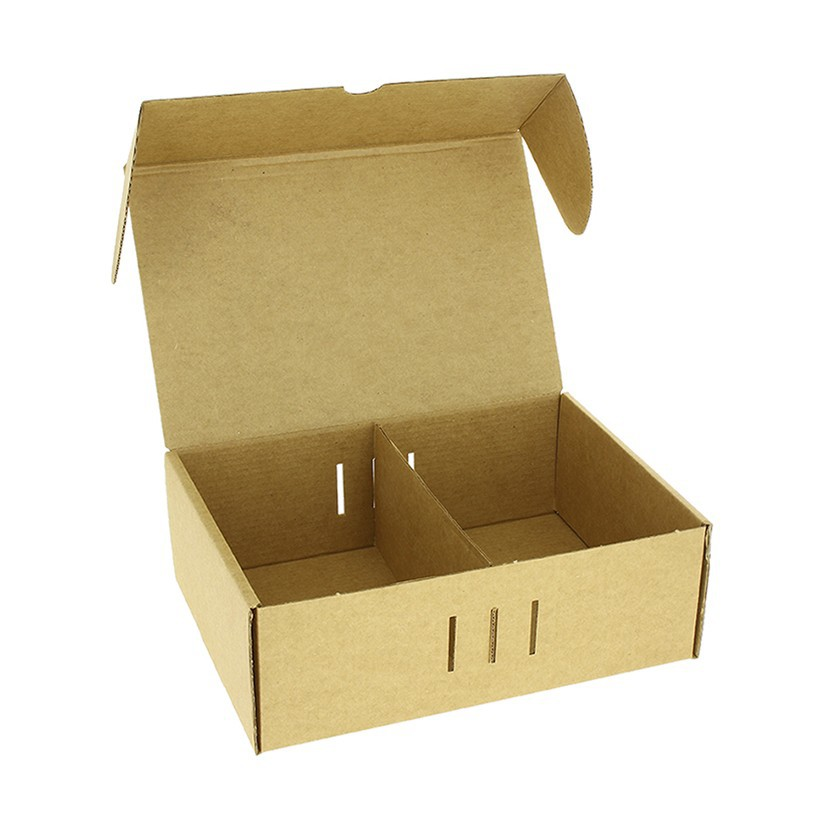
\includegraphics[width=0.75\linewidth]{00_Modificacion/Divisiones.jpg}    
\end{center}
\end{columns}

\column{0.40\linewidth}

\begin{center}
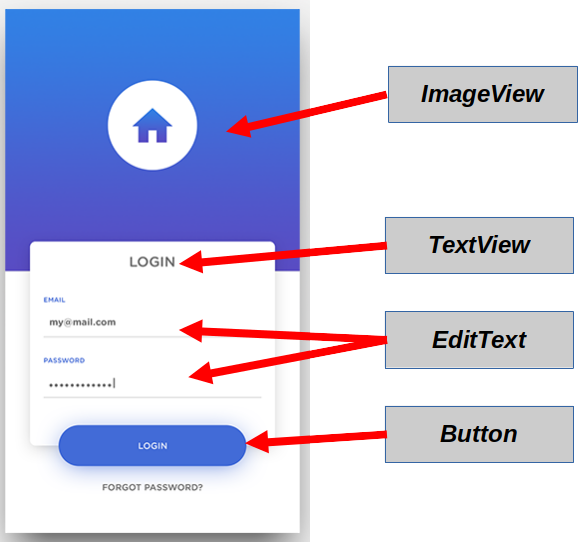
\includegraphics[width=0.95\linewidth]{00_Modificacion/ElementosInterfaz.png}    
\end{center}

\end{columns}

\end{frame}


\begin{frame}[fragile]
\frametitle{Primer modificaci\'on}

\begin{columns}
\column{0.48\linewidth}
\begin{block}{Archivo Original \textbf{activity\_main.xml}}
\begin{minted}[highlightlines={2,10,13-17},linenos,fontsize=\tiny]{xml}
<?xml version="1.0" encoding="utf-8"?>
<androidx.constraintlayout.widget.ConstraintLayout 
    xmlns:android="http://schemas.android.com/apk/res/android"
    xmlns:app="http://schemas.android.com/apk/res-auto"
    xmlns:tools="http://schemas.android.com/tools"
    android:layout_width="match_parent"
    android:layout_height="match_parent"
    tools:context=".MainActivity">
    <TextView
        android:layout_width="wrap_content"
        android:layout_height="wrap_content"
        android:text="Hello World!"
        app:layout_constraintBottom_toBottomOf="parent"
        app:layout_constraintEnd_toEndOf="parent"
        app:layout_constraintStart_toStartOf="parent"
        app:layout_constraintTop_toTopOf="parent" />
</androidx.constraintlayout.widget.ConstraintLayout>
\end{minted}
\end{block}
\column{0.48\linewidth}
\begin{block}{Archivo Modificado \textbf{activity\_main.xml}}
\begin{minted}[highlightlines={2,15,8,11,12},linenos,fontsize=\tiny]{xml}
<?xml version="1.0" encoding="utf-8"?>
<LinearLayout
    xmlns:android="http://schemas.android.com/apk/res/android"
    xmlns:app="http://schemas.android.com/apk/res-auto"
    xmlns:tools="http://schemas.android.com/tools"
    android:layout_width="match_parent"
    android:layout_height="match_parent"
    android:orientation="vertical"
    tools:context=".MainActivity">
    <TextView
        android:background="#00ffff"
        android:layout_width="match_parent"
        android:layout_height="wrap_content"
        android:text="Hello World!" />
</LinearLayout>
\end{minted}
\end{block}
\end{columns}
\end{frame}




\begin{frame}[fragile]
\frametitle{Primer modificaci\'on}

\begin{columns}
\column{0.80\linewidth}
\begin{enumerate}
\item Reemplazar \textit{androidx.constraintlayout.widget.ConstraintLayout} por \textit{LinearLayout}
\begin{itemize}
\item Tipo de contenedor donde los componentes se agregan secuencialmente
\end{itemize}
\item Agregar propiedad \textit{android:orientation=``vertical''} al \textit{LinearLayout} principal
\begin{itemize}
\item Los componentes seran ordenados verticalmente
\end{itemize}
\item Cambiar la propiedad \textit{android:layout\_width="wrap\_content"} por \textit{android:layout\_width=``match\_parent''}
\begin{itemize}
\item El ancho de TextView abarcar toda la pantalla
\end{itemize}
\item Agregar la propiedad \textit{android:background=``\#00ffff'' al textview} - 
\begin{itemize}
\item La cadena ``\#00ffff'' define el color azul. Se pueden probar con otros buscando en Internet un generador de colores hexadecimal y cambiando por otros de tu preferencia
\end{itemize}
\end{enumerate}
\column{0.20\linewidth}

\begin{center}
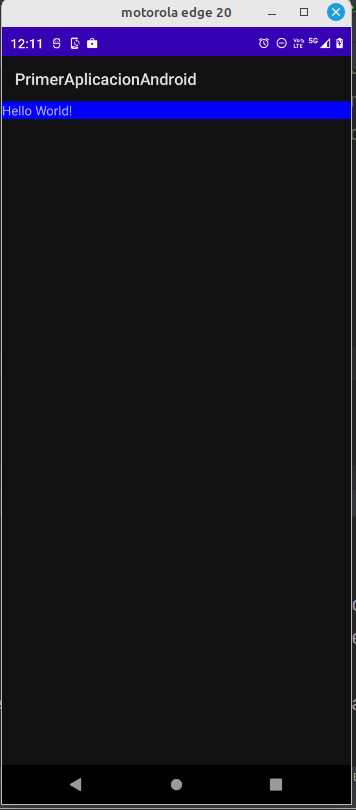
\includegraphics[width=0.95\linewidth]{00_Modificacion/App_Version2.png}    
\end{center}
\end{columns}
\end{frame}
